\section{Sharpening Turns Interpretive Uncertainty into Assumptions and Declines}
\label{sec:accommodation}

\paragraph{Accuracy hides a rise in self-consistent answers.} Qwen3-4B-Base answers 28\% of unanswerable UMWP questions self-consistently; after three rounds, 41--48\% (all five seeds; Figures~\ref{fig:overview}d and~\ref{fig:teaser}b). Stricter thresholds give the same picture (six of eight samples: 9\% to 18--23\%; all eight: 0.5\% to 3.5--7.5\%$^{\dagger}$; Appendix~\ref{app:readings}). Qwen3-8B goes from 26\% to 34--38\%, and Phi-4-mini from 21\% to 53--55\%, partly through answer formatting (two thirds of its base samples give no numeric answer). For Qwen3-4B, benchmark accuracy gains 5--7 points in round one and at most 2.5 more by round three, and accuracy on the answerable UMWP originals rises from 92\% to 95--97\%; neither reveals the change. The ill-posed problems neither drive nor markedly hold back the benchmark gain: removing them changes it by $+0.4$ to $+0.8$ points (Table~\ref{tab:attribution}).

\begin{table}[t]
\centering
\footnotesize
\setlength{\tabcolsep}{2pt}
\resizebox{\columnwidth}{!}{%
\begin{tabular}{lcccc}
\toprule
Contrast (seeds) & Items & \begin{tabular}[b]{@{}c@{}}Planted\\deletions\end{tabular} & $\Delta$SC (95\% CI) & $\Delta$Acc \\
\midrule
Solvable only (4) & 142 ($-76\%$) & $-102$ & $-5.3$ {\scriptsize$[-8.6, -1.9]$} & $+0.4$ \\
Same size$^{\dagger}$ (5) & 148--177 (0) & $-30$ & $-0.4$ {\scriptsize$[-2.9, 2.1]$} & $+0.8$ \\
Same size, no planted (5) & 148--177 (0) & $0$ & $-0.1$ {\scriptsize$[-3.6, 3.4]$} & $+0.5$ \\
Size-matched random loop$^{\dagger}$ (3) & 397 ($-33\%$) & $-33$ & $+3.8$ {\scriptsize$[0.6, 7.1]$} & $-0.1$ \\
\bottomrule
\end{tabular}}
\caption{Where the self-consistent answers come from (Qwen3-4B, round 3, UMWP). Items: size of the smaller set (seed mean or range) and its change relative to the larger one; other columns: seed-level paired differences in admitted planted premise-deleted problems, self-consistent-answer rate (SC; points; $t$-interval) and accuracy. Same size: one round from the round-2 solver on the solvable admitted problems or an equally large random subset, whose planted deleted problems the next row replaces with other admitted proposals. Last row: a loop admitting a guard-sized random subset of the band (\S\ref{sec:remedies}).}
\label{tab:attribution}
\end{table}

\paragraph{Most of the rise is sharpening.} A Qwen3-4B curriculum of only admitted problems labelled solvable still reaches 38--40\% at round three. Removing ill-posed problems lowers the rate in all four seeds, by 5 points on average (Table~\ref{tab:attribution}), but it also discards all planted premise-deleted problems and three quarters of the training set, which is then seen more often (11--15 passes per problem, against 3.3). Holding size and passes fixed, one round on the solvable problems instead of an equally large random subset, which holds 79--95 more ill-posed proposals and 20--39 planted premise-deleted problems, changes the rate by only $-0.4$ points (95\% CI $[-2.9, 2.1]$; lower in three of five seeds$^{\dagger}$); with the planted problems replaced by other random admitted proposals, the difference is $-0.1$ points ($[-3.6, 3.4]$), and putting them back adds $+0.3$ ($[-3.0, 3.6]$). At matched size we thus detect no contribution of the ill-posed or planted problems; whether they add to the sharpening that any label-free curriculum shares is not established at five seeds.

\begin{figure}[t]
\centering
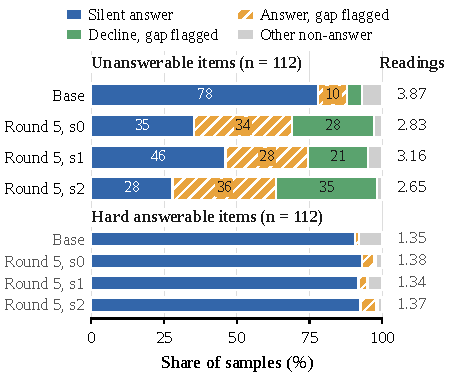
\includegraphics[width=0.83\columnwidth]{figures/fig3_accommodation.pdf}
\caption{How Qwen3-4B answers 112 unanswerable and 112 hard answerable UMWP questions at base and round 5 (eight samples each; gap flags from blind LLM labellers, answers read as in \S\ref{sec:setting}): shares of samples that answer silently, answer while flagging a gap or stating an assumption$^{\dagger}$, decline while flagging a gap, or give no answer otherwise, and mean number of readings. Human annotators confirm the rise in flagged samples (Appendix~\ref{app:readings}).}
\label{fig:accommodation}
\end{figure}

\paragraph{Sharpening turns scattered guesses into stated assumptions and declines.} The base model rarely declines: 88\% of its samples on unanswerable questions give a number, 78\% without comment, and they scatter (Figure~\ref{fig:accommodation}). After five rounds, 49--70\% of the solver's samples state an assumption or flag a gap, against 15\% at base (human annotators: 14\% to 58\%): 28--36\% still answer, on a stated assumption, and 21--35\% decline in words, while 28--46\% answer silently$^{\dagger}$ (human annotators: 30\%, 28\% and 40\%). Questions answered self-consistently with no sample flagging a gap stay at 5--8\%$^{\dagger}$. The rise is overt accommodation, not silent confabulation, and comes with more declines; a stated assumption lets a reader catch the defect, but not a pipeline that reads only the final number, nor our self-consistency rate. Seeds converge on the same assumption, mostly the base model's preference$^{\dagger}$: on the 205 unanswerable questions all three round-5 seeds answer self-consistently, they agree on 88\% (three base-model runs: 66\%), and on 78\% of these (86\% counting ties) their answer is the base model's mode.

\paragraph{Precedent fills the gap.} Whatever the defect, the solver accommodates \citep{lewis1979scorekeeping} the question's presupposition that it has a unique answer \citep{karttunen1977questions,belnap1976questions}: it picks a reading, supplies a missing value or drops a conflicting condition. The majority-vote reward makes the eight samples a coordination problem that self-play settles by a convention \citep{lewis1969convention} selected by precedent, with the base model's preference as the focal point \citep{schelling1960strategy}: training mostly makes the assumption the consensus rather than inventing it.

\paragraph{Offered a way out, the solver takes it.} Without the option, the round-3 solvers decline in words in 13--22\% of their samples on unanswerable UMWP questions (base model: 3\%). Given the option to answer \texttt{unknown}, the drifted and solvable-only curricula abstain at the same rate, 69--71\% at round three (seeds 0--3; base model 53\%), with about 2\% false abstention (base: 5\%); on SUM, MiP-GSM8K and MiP-MATH \citep{song2025hallucination,fan2025mip} they abstain within 0.05 of each other in 11 of 12 seed-level comparisons, whereas without the option the drifted curriculum answers self-consistently more often in ten of the twelve. Self-play training does not remove the ability to recognise an unanswerable question; it changes what the model does when no one asks.
